%-------------------------------------------------------------------------------
%	PACKAGES AND OTHER DOCUMENT CONFIGURATIONS
%-------------------------------------------------------------------------------

\documentclass{article}

% Packages
% Packages

% \usepackage{fancyhdr} % Required for custom headers
% \usepackage{lastpage} % Required to determine the last page for the footer
% \usepackage{extramarks} % Required for headers and footers
% \usepackage[usenames,dvipsnames]{color} % Required for custom colors
\usepackage{graphicx} % Required to insert images
% \usepackage{listings} % Required for insertion of code
% \usepackage{courier} % Required for the courier font
% \usepackage{dsfont} % For special math characters
% \usepackage{verbatim}

%\usepackage{amsmath, amssymb, bm} % For matrix notation
\usepackage[english]{babel}
\usepackage[paperwidth=8.5in,paperheight=11in,margin=1.0in]{geometry}
\usepackage{listings}
\usepackage{hyperref}
%\usepackage[cmex10]{amsmath, bm}
\usepackage{amsmath, bm}
\usepackage{blkarray}








% formatting
\pdfcompresslevel0

% ==============================================================================
% PYTHON
% ==============================================================================
\usepackage[utf8]{inputenc}

% Default fixed font does not support bold face
\DeclareFixedFont{\ttb}{T1}{txtt}{bx}{n}{12} % for bold
\DeclareFixedFont{\ttm}{T1}{txtt}{m}{n}{12}  % for normal

% Custom colors
\usepackage{color}
\definecolor{deepblue}{rgb}{0,0,0.5}
\definecolor{deepred}{rgb}{0.6,0,0}
\definecolor{deepgreen}{rgb}{0,0.5,0}

\usepackage{listings}

% Python style for highlighting
\newcommand\pythonstyle{\lstset{
language=Python,
basicstyle=\ttm,
otherkeywords={self},             % Add keywords here
keywordstyle=\ttb\color{deepblue},
emph={MyClass,__init__},          % Custom highlighting
emphstyle=\ttb\color{deepred},    % Custom highlighting style
stringstyle=\color{deepgreen},
frame=tb,                         % Any extra options here
showstringspaces=false,            % 
breaklines=true
}}


% Python environment
\lstnewenvironment{python}[1][]
{\pythonstyle\lstset{#1}
}
{}

% Python for external files
\newcommand\pythonexternal[2][]{{
\pythonstyle\lstinputlisting[#1]{#2}}}

% Python for inline
\newcommand\pythoninline[1]{{\pythonstyle\lstinline!#1!}}
% ==============================================================================
% ==============================================================================

% Margins
\topmargin=-0.45in
\evensidemargin=0in
\oddsidemargin=0in
\textwidth=6.5in
\textheight=9.0in
\headsep=0.25in

\linespread{1.1} % Line spacing

% Set up the header and footer
\pagestyle{fancy}
\lhead{\hmwkAuthorName} % Top left header
\chead{\hmwkClass\ (\hmwkClassInstructor\ \hmwkClassTime): \hmwkTitle} % Top center head
\rhead{\firstxmark} % Top right header
\lfoot{\lastxmark} % Bottom left footer
\cfoot{} % Bottom center footer
\rfoot{Page\ \thepage\ of\ \protect\pageref{LastPage}} % Bottom right footer
\renewcommand\headrulewidth{0.4pt} % Size of the header rule
\renewcommand\footrulewidth{0.4pt} % Size of the footer rule

\setlength\parindent{0pt} % Removes all indentation from paragraphs

%----------------------------------------------------------------------------------------
%	DOCUMENT STRUCTURE COMMANDS
%	Skip this unless you know what you're doing
%----------------------------------------------------------------------------------------

% Header and footer for when a page split occurs within a problem environment
\newcommand{\enterProblemHeader}[1]{\nobreak\extramarks{#1}{#1 continued on next page\ldots}\nobreak\nobreak\extramarks{#1 (continued)}{#1 continued on next page\ldots}\nobreak}

% Header and footer for when a page split occurs between problem environments
\newcommand{\exitProblemHeader}[1]{\nobreak\extramarks{#1 (continued)}{#1 continued on next page\ldots}\nobreak\nobreak\extramarks{#1}{}\nobreak}

\setcounter{secnumdepth}{0} % Removes default section numbers
\newcounter{homeworkProblemCounter} % Creates a counter to keep track of the number of problems

\newcommand{\homeworkProblemName}{}
\newenvironment{homeworkProblem}[1][Problem \arabic{homeworkProblemCounter}]{ % Makes a new environment called homeworkProblem which takes 1 argument (custom name) but the default is "Problem #"
\stepcounter{homeworkProblemCounter} % Increase counter for number of problems
\renewcommand{\homeworkProblemName}{#1} % Assign \homeworkProblemName the name of the problem
\section{\homeworkProblemName} % Make a section in the document with the custom problem count
\enterProblemHeader{\homeworkProblemName} % Header and footer within the environment
}{\exitProblemHeader{\homeworkProblemName} % Header and footer after the environment
}

% Defines the problem answer command with the content as the only argument
\newcommand{\problemAnswer}[1]{\noindent\framebox[\columnwidth, resolution=600][c]{\begin{minipage}{0.98\columnwidth, resolution=600}#1\end{minipage}}}
% Makes the box around the problem answer and puts the content inside }

\newcommand{\homeworkSectionName}{}
\newenvironment{homeworkSection}[1]{ % New environment for sections within homework problems, takes 1 argument - the name of the section
\renewcommand{\homeworkSectionName}{#1} % Assign \homeworkSectionName to the name of the section from the environment argument
\subsection{\homeworkSectionName} % Make a subsection with the custom name of the subsection
\enterProblemHeader{\homeworkProblemName\ [\homeworkSectionName]} % Header and footer within the environment
}{
\enterProblemHeader{\homeworkProblemName} % Header and footer after the environment
}



%----------------------------------------------------------------------------------------
%	NAME AND CLASS SECTION
%----------------------------------------------------------------------------------------

\newcommand{\hmwkTitle}{Homework 2} % Assignment title
\newcommand{\hmwkDueDate}{Friday, Sept. 25} % Due date
\newcommand{\hmwkClass}{ECE 532} % Course/class
\newcommand{\hmwkClassTime}{11:00 am} % Class/lecture time
\newcommand{\hmwkClassInstructor}{Robert Nowak} % Teacher/lecturer
\newcommand{\hmwkAuthorName}{Elijah Bernstein-Cooper} % Your name

%-------------------------------------------------------------------------------
%	TITLE PAGE
%-------------------------------------------------------------------------------

\title{\vspace{0in}
    \textmd{\textbf{\hmwkClass:\ \hmwkTitle}}\\
    \normalsize\vspace{0.1in}\small{Due\ on\ \hmwkDueDate}\\
    \vspace{0.1in}\large{\textit{\hmwkClassInstructor\ \hmwkClassTime}}
    \vspace{0.5in}}

\author{\textbf{Elijah Bernstein-Cooper}}
\date{\today} % Insert date here if you want it to appear below your name

%-------------------------------------------------------------------------------

\begin{document}

\maketitle
%\newpage

%===============================================================================
%-------------------------------------------------------------------------------
%	PROBLEM 1
%-------------------------------------------------------------------------------
\begin{homeworkProblem}

    \begin{homeworkSection}{1a}
        
        We know that for an overdetermined system, the least squares solution
        to the matrix $\bm{\hat{x}}$ will be 

        \begin{equation*}
            {(\bm{A}^T \bm{A})}^{-1}\bm{A}^T\bm{b}
        \end{equation*}

        \noindent which gives us

        \begin{equation*}
            \bm{\hat{x}} = 
                0.75 \left(\begin{matrix} 1 \\ 1 \\ 1 \end{matrix}\right) + 
                0.25 \left(\begin{matrix} 1 \\ -1 \\ 1 \end{matrix}\right)
        \end{equation*}

    \end{homeworkSection}

    \begin{homeworkSection}{1b}
        
        See Figure~\ref{fig:1b} for a sketch of the problem.

        \begin{figure}[!ht]
            \begin{centering}

            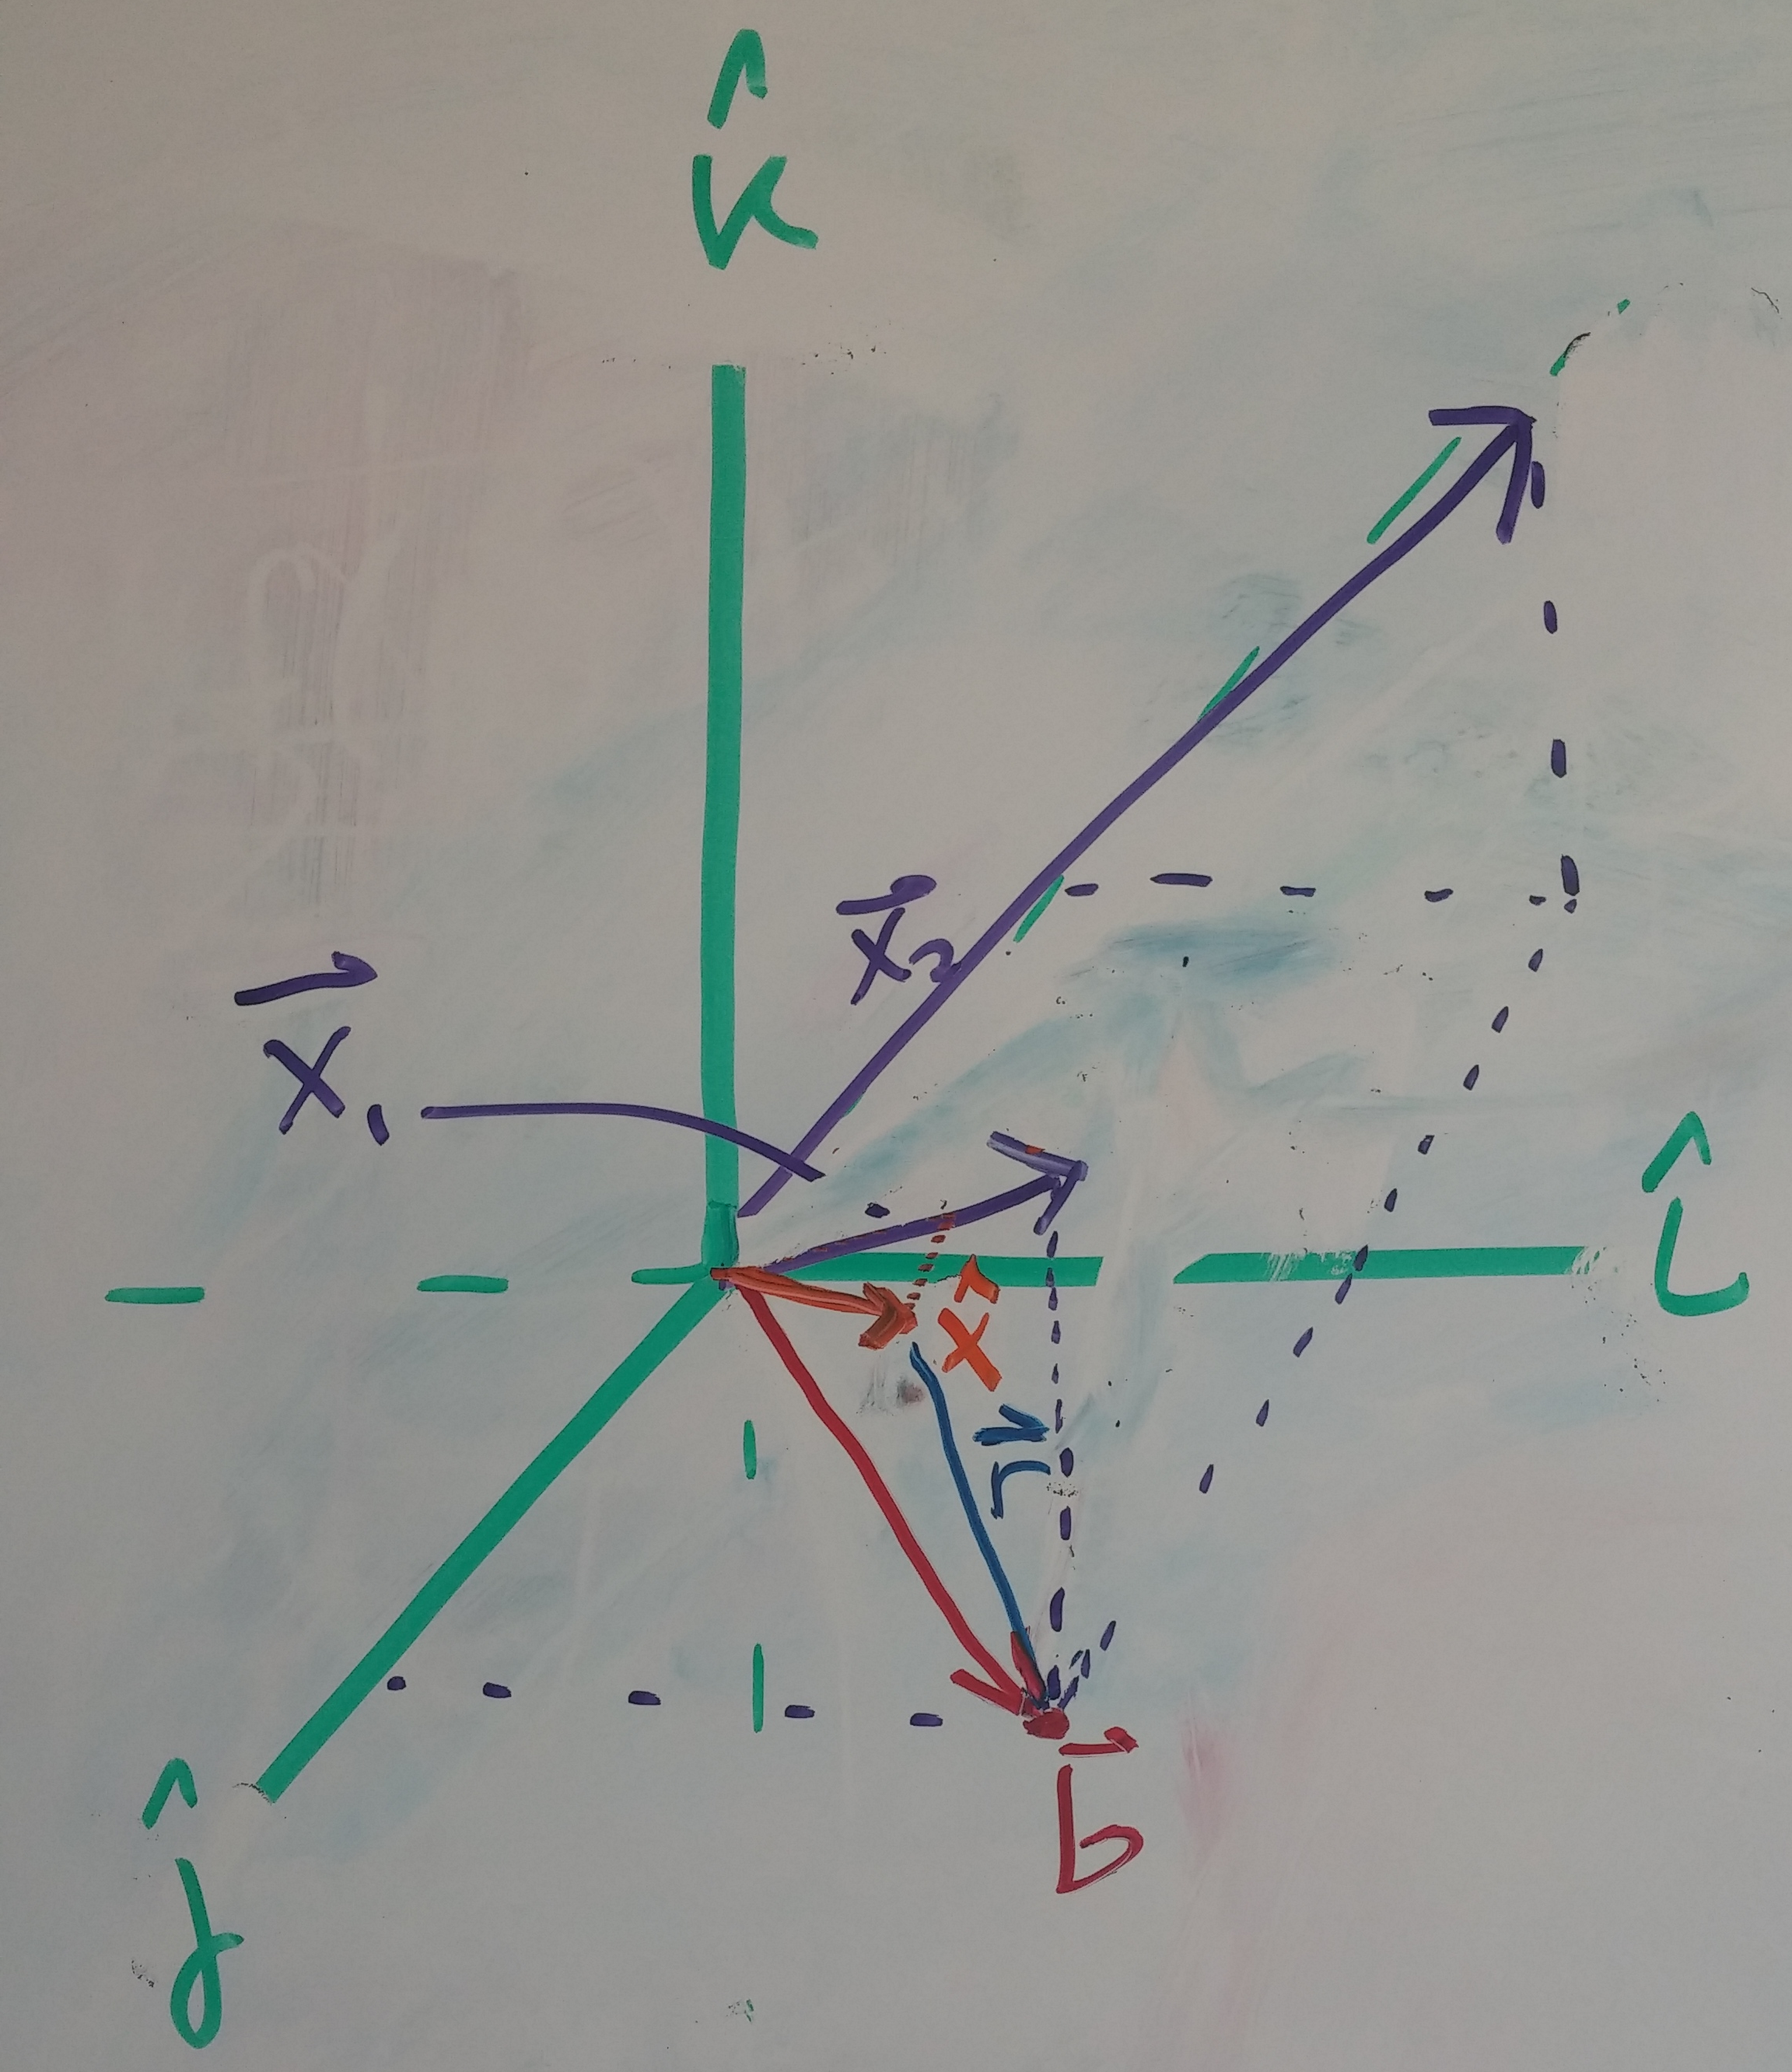
\includegraphics[scale=0.08]{problem1b_fig.png}

            \caption{\label{fig:1b} Sketch of $\bm{A}$ and $\bm{b}$.}

            \end{centering}
        \end{figure}

    \end{homeworkSection}

\end{homeworkProblem}
%\clearpage
%===============================================================================

%===============================================================================
%-------------------------------------------------------------------------------
%	PROBLEM 2 
%-------------------------------------------------------------------------------
\begin{homeworkProblem}

    \begin{homeworkSection}{2a}
        
        The matrix A will be a $m \times 2$ matrix consisting of the measured
        responses for each condition in $m$ experiments.

    \end{homeworkSection}

    \begin{homeworkSection}{2c}

                See Figure~\ref{fig:2c}.

        \begin{figure}[!ht]
            \begin{centering}
            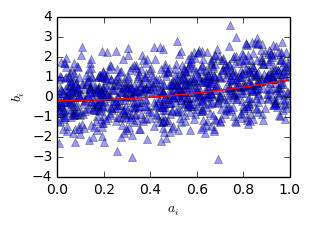
\includegraphics[scale=1]{problem2c_fig.png}

            \caption{\label{fig:2c} $\bm{A}$ and $\bm{b}$.}
            
            \end{centering}
        \end{figure}

    \end{homeworkSection}

    \begin{homeworkSection}{2d}

                See Figure~\ref{fig:2d}.

        \begin{figure}[!ht]
        \begin{centering}
            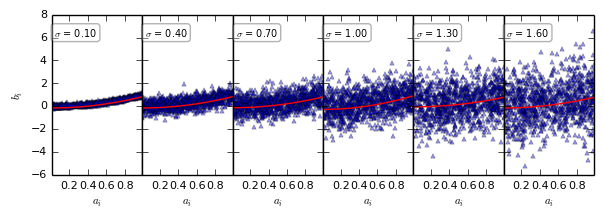
\includegraphics[scale=1]{problem2d_fig.png}

            \caption{\label{fig:2d} $\bm{A}$ and $\bm{b}$.}

        \end{centering}
        \end{figure}

    \end{homeworkSection}

\end{homeworkProblem}
%===============================================================================

%===============================================================================
%-------------------------------------------------------------------------------
%	PROBLEM 3
%-------------------------------------------------------------------------------
\begin{homeworkProblem}

    \begin{homeworkSection}{3a}

        To find min$_{\bm{x}} \|\tilde{\bm{A}}\bm{x} - \tilde{\bm{b}}\|_2$ we
        know that the expression will be smallest when the difference inside
        the norm is equal to 0. Thus our problem becomes solving the linear
        equation

        \begin{equation*}
            \tilde{\bm{A}}\bm{x} = \tilde{\bm{b}}
        \end{equation*}

        \noindent for $\bm{x}$ for which there is the well-known solution

        \begin{equation*} 
            (\tilde{\bm{A}}^T \tilde{\bm{A}})^{-1}
            \tilde{\bm{A}}^T \tilde{\bm{b}} = \bm{x}
        \end{equation*}

    \end{homeworkSection}

    \begin{homeworkSection}{3b}
       
        See Figure~\ref{fig:3b} and the following code
        \pythonexternal{hw3.m}

        \begin{figure}[!ht]
        \begin{centering}
            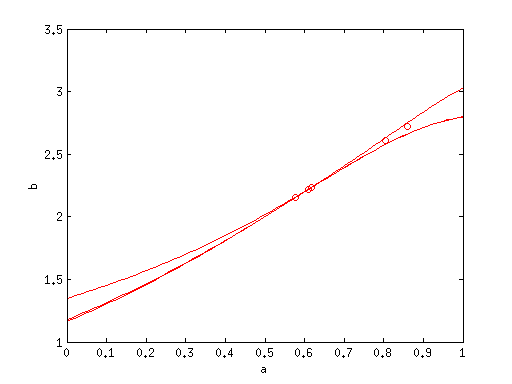
\includegraphics[scale=1]{problem3c_fig.png}

            \caption{\label{fig:3b} Plot of data with fitted 9th degree
            polynomial with varying values of $\epsilon$.}

        \end{centering}
        \end{figure}

    \end{homeworkSection}

    \begin{homeworkSection}{3c}
        See Figure~\ref{fig:3b}.
    \end{homeworkSection}

\end{homeworkProblem}
%===============================================================================

%===============================================================================
%-------------------------------------------------------------------------------
%	PROBLEM 4
%-------------------------------------------------------------------------------
\begin{homeworkProblem}

    \begin{homeworkSection}{4a}

        By solving the linear equation

        \begin{equation*}
            \bm{A x} = \bm{b}
        \end{equation*}

        \noindent we obtain a set of weights $\bm{x}$ where

        \begin{equation*}
            \bm{x} = \left(\begin{matrix}
                             0.943 \\
                             0.213 \\
                             0.266 \\
                            -0.392 \\
                            -0.005 \\
                            -0.017 \\
                            -0.166 \\
                            -0.082 \\
                            -0.166 \\
          \end{matrix}\right)       
        \end{equation*}

    \end{homeworkSection}

    \begin{homeworkSection}{4b}

        To classify a new face as happy or mad we would multiply the new data
        matrix $\bm{a}_i$ by the weights. If the product is greater than 0,
        then the face is happy, if the product is less than 0, the face is
        mad.

    \end{homeworkSection}

    \begin{homeworkSection}{4c}

        Feature 1 best determines a happy face because it has the largest
        positive weight, while feature 4 best determines a mad face because it
        has the smallest negative weight. 

    \end{homeworkSection}

    \begin{homeworkSection}{4d}
        
        To build a classifier out of just three features we will use the
        features with the largest absolute value weight, at least one feature
        for happy and mad (positive and negative weights) and attempt to
        minimize the difference between the sum of the absolute values of
        weights for happy and mad features. The final criterion allows us to
        compromise our accuracy for determining a happy face or a mad face. \\

        These criteria lead us to choose features 1, 4, and 9 as the three most
        important features for determining a happy or a mad face. We would
        build a classifier in the same way as in Problem \S 4b, except using
        only features 1, 4, and 9.

    \end{homeworkSection}
    
    \begin{homeworkSection}{4e}
        
        Please see the code under the function 4e at the end of the homework.

    \end{homeworkSection}
    
    \begin{homeworkSection}{4f}

        Errors with 9 features: \\
            False positives = 0.507 \\
            False negatives = 0.492 \\ \\

        Errors with 3 features: \\
            False positives = 0.507 \\
            False negatives = 0.492 \\ \\

        We can see that using three features works just as well as using the
        nine features.

    \end{homeworkSection}

\end{homeworkProblem}
%===============================================================================

\begin{homeworkProblem}
    \pythonexternal{hw3.py}
\end{homeworkProblem}

\end{document}

